\chapter{Printing Your Thesis}
\label{cha:Printing}


\section{PDF Workflow}
\label{sec:pdf-workflow}

Nowadays \latex\ is practically always used in such a way that it creates PDF
documents directly (without the detour via DVI and PostScript that was common
in the past). In modern environments (\eg, \emph{TeXstudio} or \emph{Overleaf})
this works automatically without any further configuration effort.


\subsection{PDF Archive Format (PDF/A)}
\label{sec:PDFA}

Many institutions require theses to be submitted in PDF/A format, which is a
standardized variant of PDF for archiving and long-term preservation.%
\footnote{\url{https://en.wikipedia.org/wiki/PDF/A}}
This document is rendered in PDF/A format by default (PDF/A-2b to be exact),
caused by
%
\begin{LaTeXCode}[numbers=none]
\RequirePackage{hgbpdfa}
\end{LaTeXCode}
%
at the beginning of file \verb!main.tex! (loading \verb!hgbpdfa.sty!).
Note that this must be placed \emph{before} the \verb!\begin{document}!
statement. Required meta-data (\eg, author and title) are automatically 
derived from the document settings and inserted into the output PDF.%
\footnote{This setup builds on new functionality currently being added to
the \texttt{pdflatex} kernel and requires package \texttt{pdfmanagement-testphase}
version 0.95s (2022-09-26) or higher. With older versions (\eg, on \emph{Overleaf}
at this time), a package warning is issued and no PDF/A is produced.}


\subsection{PDF/A Issues}
\label{sec:PDFA-issues}

Activating the PDF/A option creates an output file that \emph{claims} to be 
PDF/A-compliant but this does not imply that is actually \emph{is}.
Although \emph{this} document produces a compliant PDF/A, any derived document
may not do so. It is therefore important to \emph{validate} the resulting PDF file
before submission using one of the options described below. Most violations
of the PDF/A standard arise from the inclusion of other PDF files, particularly 
graphics. Typical issues are related to the use of non-embedded fonts
and incorrect or unwanted color spaces. This setup assumes sRGB colors, 
which should also be used when creating your own illustrations.

Problems with imported PDF files may be difficult to locate in the final (composite)
document. Once the troubling file is known and cannot be regenerated, it may be fixed using 
other tools such as Adobe \emph{Acrobat} (\emph{Distiller}) or \emph{Ghostscript}.%
\footnote{\url{https://ghostscript.com/}}


\subsection{PDF/A Validation}
\label{sec:PDFA-validation}

A straightforward (and free) method to validate PDF/A compliance is provided by
\textsf{veraPDF}, which includes
%
\begin{itemize}
\item an open-source validation client%
  \footnote{\url{https://verapdf.org/software} (Windows, macOS, Linux)} and
\item an online validation service.%
  \footnote{\url{https://demo.verapdf.org}}
\end{itemize}
%
See Figure \ref{fig:verapdf-report} for an example.
A similar service is offered by \textsf{pdf-online.com},%
\footnote{\url{https://www.pdf-online.com/osa/validate.aspx}}
unfortunately announced to be retired in 2023.
Of course, PDF/A validation is also contained in the toolset of Adobe \emph{Acrobat}.

\begin{figure}[htbp]
    \centering
    \fbox{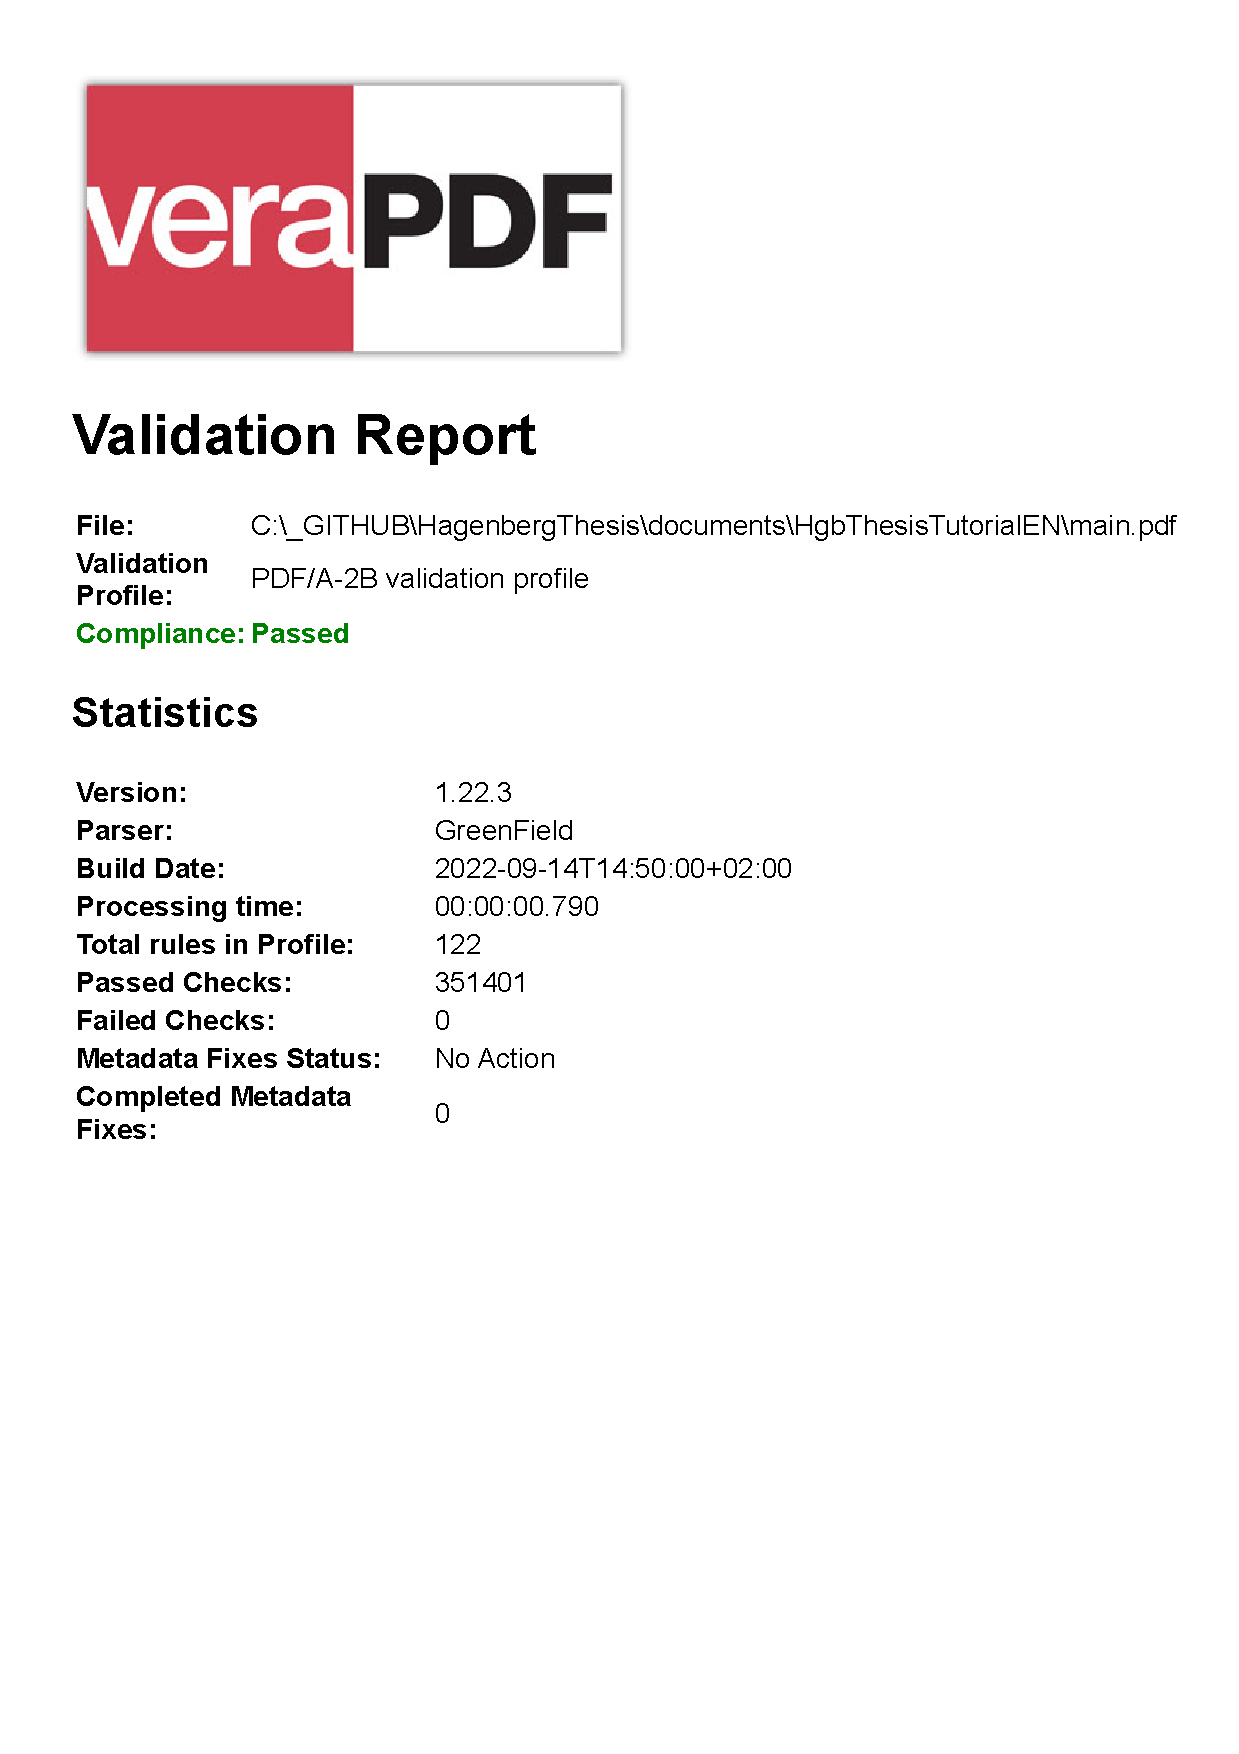
\includegraphics[width=.60\textwidth]{verapdf-report}}
    \caption{Report produced by the \textsf{veraPDF} client after successful validation
    of \emph{this} document. Note that this screenshot was imported as a PDF 
    which itself is \emph{not} PDF/A-compliant.}
    \label{fig:verapdf-report}
\end{figure}



\section{Printing}

Before printing the manuscript, it is advisable to consider a few things in
order to avoid unnecessary trouble (and costs).


\subsection{Printer and Paper}

It is essential that the final version of the thesis be printed on a high-quality
\emph{laser printer}; printouts made with inkjet printers are \emph{not} sufficient.
The paper used should also be of good quality (woodfree) and usual thickness 
(typ.\ $80\,\mathrm{g} / \mathrm{m}^2$). If only a few \emph{color} pages are
necessary, one may print them separately on a color laser printer and insert
them into the main document (printed in black and white).

By the way, \emph{all} copies to be handed in should be \emph{printed} (and not 
copied)! The cost of printing is no higher than that of copies, but the difference
in quality is---especially for pictures and graphics---usually significant.


\subsection{Print Size}

First of all, make sure that the paper size set in the final PDF file is really
\textrm{A4}! This can be done, for example, with Adobe \emph{Acrobat} or 
\emph{SumatraPDF} via \texttt{File} $\rightarrow$ \texttt{Properties} 
to show the document's paper size:
%
\begin{center}
	\textrm{Correct:} A4 = $8{,}27 \times 11{,}69$ inches or $210 \times 297$ mm.
\end{center}
%
If this does not match, then probably "Letter" is set as the paper size somewhere
in the workflow by mistake.

A common and easily overlooked error when printing PDF documents is caused by 
accidentally setting the "Fit to page" option in the print menu, usually printing 
pages that are too small. Therefore, make sure you check the size of the printout 
by verifying the text width%
\footnote{\Convert[unit=mm]{\the\textwidth}	in this document.} % using 'lengthconvert' package
or using the measurement frame included at the end of this document.
To be on the safe side, this measurement frame should be kept until the work 
is completed, and only then the corresponding page should be removed.
If, as mentioned before, individual color pages are printed separately, these 
should of course also be checked carefully for compliance with the print size!


\section{Binding the Manuscript}

The final version of the thesis must be submitted in hard bound form.%
\footnote{For a \emph{bachelor} thesis, depending on the requirements of the study
program, a simple binding (\eg, by a good copy store) is usually sufficient.}
A binding must be used that permanently prevents individual pages from falling out,
\eg, by means of a traditional spine binding (bookbinder) or by means of 
commercially available plastic or metal staples.%
\footnote{At the Faculty of Hagenberg, at least one of the copies of a master's
thesis is to be handed in unbound---this is later bound by a bookbinder in a
uniform form and then remains in the library.}
If you have the work done by a professional bookbinder, which is highly recommended,
you should also pay attention to the \emph{embossing on the spine}, since
it increases the cost only slightly. It is common to include the surname of the author
and the title of the thesis. If the name and/or title is too long, you should specify
a shortened version if necessary, such as:
%
\begin{center}
	\setlength{\fboxsep}{3mm}
	\fbox{\textsc{Wiseguy}
		\textperiodcentered\ \textsc{Part. Solutions to Univ. Problems}}
\end{center}
%
After binding, be sure to check the final work once more for completeness, correct 
arrangement of pages, etc.



\begin{comment}	% this is outdated
\section{Elektronische Datenträger (CD-R, DVD)}

Speziell bei Arbeiten im Bereich der Informationstechnik (aber nicht nur
dort) fallen fast immer Informationen an, wie Programme, Daten, Grafiken,
Kopien von Internetseiten \usw, die für eine spätere Verwendung elektronisch
verfügbar sein sollten. Vernünftigerweise wird man diese Daten während der
Arbeit bereits gezielt sammeln und der fertigen Arbeit auf einer CD-ROM oder
DVD beilegen.%
\footnote{Als Alternative sehen Institute zunehmend den Upload dieser Daten
in ein entsprechendes Online-Archiv vor, zumal CD/DVD-Laufwerke in neuen
Geräten kaum mehr eingebaut werden. Das konkrete Vorgehen sollte man
jedenfalls mit den zuständigen Stellen abstimmen.}
Es ist außerdem sinnvoll -- schon allein aus Gründen der elektronischen
Archivierbarkeit -- auch die eigene Arbeit selbst als PDF-Datei beizulegen.%
\footnote{Auch Bilder und Grafiken könnten in elektronischer Form nützlich
sein, die \latex-Dateien sind hingegen überflüssig.}

Falls ein elektronischer Datenträger (CD-ROM, DVD) beigelegt wird, sollte auf
folgende Dinge geachtet werden:
%
\begin{enumerate}
	\item Jedem abzugebenden Exemplar muss eine identische Kopie des
	Datenträgers beiliegen.
	\item Verwenden Sie qualitativ hochwertige Rohlinge und überprüfen
	Sie nach der Fertigstellung die tatsächlich gespeicherten Inhalte
	des Datenträgers!
	\item Der Datenträger sollte in eine im hinteren Umschlag eingeklebte
	Hülle eingefügt sein und sollte so zu entnehmen sein, dass die Hülle
	dabei \emph{nicht} zerstört wird (die meisten Buchbinder haben geeignete
	Hüllen parat).
	\item Der Datenträger muss so beschriftet sein, dass er der
	Abschlussarbeit eindeutig zuzuordnen ist, am Besten durch ein
	gedrucktes Label%
	\footnote{Nicht beim lose abgegebenen Bibliotheksexemplar --
	dieses erhält ein standardisiertes Label durch die Bibliothek.}
	oder sonst durch \emph{saubere}	Beschriftung mit der Hand und einem
	feinen, wasserfesten Stift.
	\item Nützlich ist auch ein (grobes) Verzeichnis der Inhalte des
	Datenträgers (wie exemplarisch in Anhang \ref{app:Materials}).
\end{enumerate}
\end{comment}